\documentclass{article}
\usepackage[UTF8]{ctex}
\usepackage{amsfonts}
\usepackage{amsmath}
\usepackage{float}
\usepackage{graphicx}
\usepackage{subcaption}
\usepackage{url}

\newcommand{\Bezier}{B\'ezier}%Bézier

\usepackage{color}

% paragraph
\setlength{\parindent}{0pt}
\setlength\parskip{\baselineskip}
\renewcommand{\baselinestretch}{1.2}

\begin{document}
	
	% 标题
	\title{《计算机辅助几何设计》作业}
	\author{ID号: 048  \qquad  姓名: 郑涛}  %递交作业时填上ID号和姓名
	\date{2024年11月28日}
	\maketitle
	1.Implement the Loop subdivision algorithm for triangle mesh. Given a low-resolution
	triangle mesh, use the Loop subdivision algorithm to perform multiple subdivisions to obtain a high-resolution smooth mesh.
	\section{Algorithm}
	\begin{figure}[H]
		\centering
		\includegraphics[scale=0.7]{"split"}
		\caption{}
		\label{fig:split}
	\end{figure}
We use 1:4 triangular splits.
	\begin{figure}[H]
		\centering
		\includegraphics[scale=0.7]{"averaging mask"}
		\caption{}
		\label{fig:averaging-mask}
	\end{figure}
	Neighbouring points and points to be updated are weighted as above when updating the position of the point,$k$ is the number of neighbours of points.The $\alpha(k)$ and $\beta(k)$ are defined as follows:
	$$\alpha(k)=\frac{k(1-\beta(k))}{\beta(k)}$$
	$$\beta(k)=\frac{5}{4}-\frac{(3+2cos(\frac{2\pi}{k}))^2}{32}$$
	
	noting that the last normalisation is performed.
	\section{Result}
	\begin{figure}[H]
		\centering
		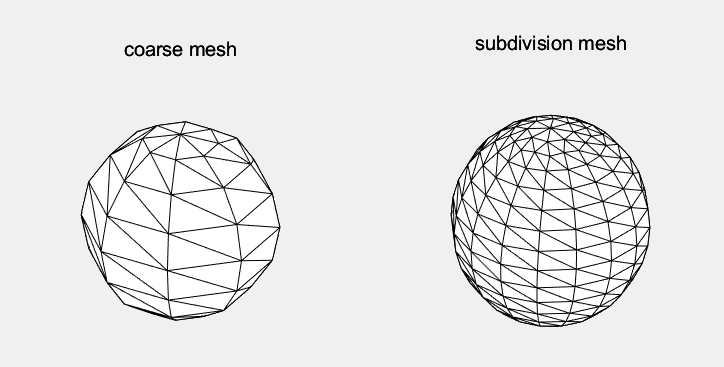
\includegraphics{1}
		\caption{loop = 1}
		\label{fig:1}
	\end{figure}
	\begin{figure}[H]
		\centering
		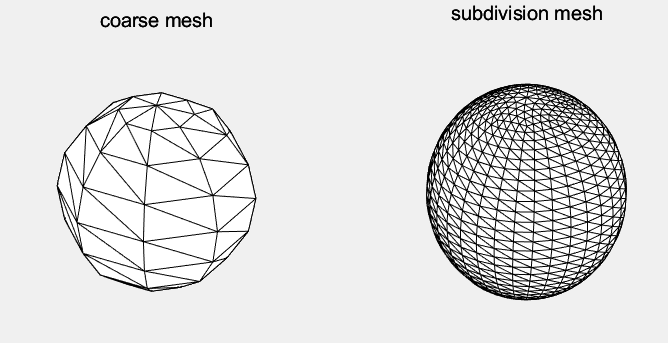
\includegraphics{2}
		\caption{loop = 2}
		\label{fig:2}
	\end{figure}
	\begin{figure}[H]
		\centering
		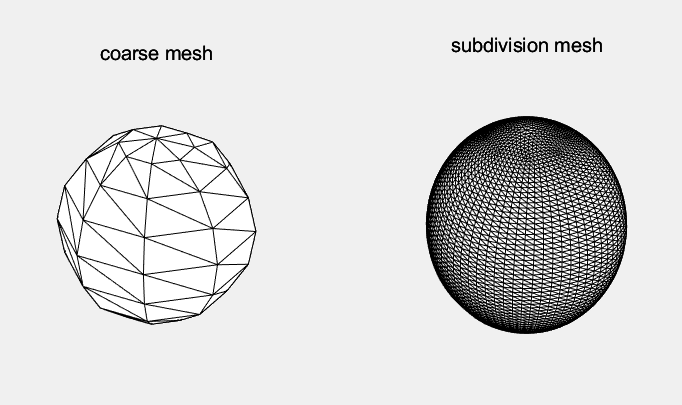
\includegraphics{3}
		\caption{loop = 3}
		\label{fig:3}
	\end{figure}
	
\end{document}











